\section{Theorie}
\label{sec:Theorie}
Analog zu der Masse bei der Translation lässt sich bei Rotationen das Trägheitsmoment definieren. Es wird dabei als Trägheit des Objektes gegenüber einer Rotation bezüglich einer Rotationsachse verstanden. Es lässt sich durch die Gleichung 
\begin{equation}
    I=\sum_{i}r_i^2\cdot m_i
\end{equation}
berechnen. $r_i$ ist dabei der Abstand des Massenelemnts $m_i$ zur Rotationsachse.
Für kontinuierliche Masseverteilungen kann zum berechnen des Trägheitsmoments die Gleichung
\begin{equation}
    I=\rho\int_V r_\perp^2 \,\symup{d}V
\end{equation}
verwendet werden. $\rho$ beschreibt die Dichte des Materials.


\begin{figure}
    \caption{Trägheitsmomente einiger Körper.}
    \centering
    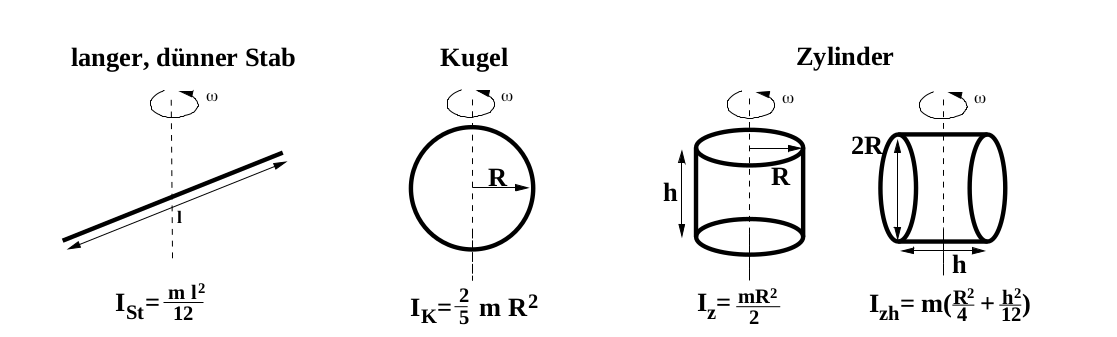
\includegraphics[height=4cm]{data/Probekoerper.png}
    \label{fig:probe}
\end{figure}


In Abbildung \ref{fig:probe} sind die in dem Versuch benötigten Trägheitsmomente aufgeführt. 
Falls die Rotationsachse um einen Abstand a zu einer parallelen Rotationsachse durch den Schwerpunkt verschoben ist, kann das Trägheitsmoment über die Gleichung
\begin{equation}
    I=I_s+m\cdot a^2
\end{equation}
berechnet werden. Diese Gleichung wird auch "Satz von Steiner" gennant.  $I_s$ ist das Trägheitsmoment bezüglich der Rotationsachse durch den Schwerpunkt.


Bei diesem Versuch wirk bei einer Drehung um den Winkel $\phi$ durch eine Torsionsfeder ein rücktreibendes Drehmoment auf das Objekt. So führt das System beim loslassen eine Schwingung um die Drehachse durch. Die Schwingungsdauer lässt sich dann über 
\begin{equation}
    T=2\pi \sqrt{\frac{I}{D}}
\end{equation}
berechnen. $D$ entspricht der Winkelrichtgröße, welche über  
\begin{equation}
    M=D\cdot \phi
\end{equation}
mit dem Drehmoment in Zusammenhang steht.
Damit die Schwingung in einem harmonischen Bereich abläuft, ist $\phi$ auf kleine Auslenkungen beschränkt.

%In knapper Form sind die physikalischen Grundlagen des Versuches, des Messverfahrens, sowie sämtliche für die Auswertung erforderlichen Gleichungen darzustellen. (Keine Herleitung)

%(eventuell die Aufgaben)

%Der Versuchsaufbau: Beschreibung des Versuchs und der Funktionsweise (mit Skizze/Bild/Foto)
